% This file is part of Bachelorarbeit

% Bachelorarbeit is free software: you can redistribute it and/or modify
% it under the terms of the GNU General Public License version 3 as published by
% the Free Software Foundation.

% Bachelorarbeit is distributed in the hope that it will be useful,
% but WITHOUT ANY WARRANTY; without even the implied warranty of
% MERCHANTABILITY or FITNESS FOR A PARTICULAR PURPOSE.  See the
% GNU General Public License for more details.

% You should have received a copy of the GNU General Public License
% along with Foobar. If not, see <http://www.gnu.org/licenses/>.
\section{Grundlage}
Um IPsec zu verstehen, müssen zuerst die Netzwerkgrundlagen verstanden werden.
\subsection{Netzwerke}
Moderne Computernetzwerke basieren auf Ethernet und \ac{IPv4} oder \ac{IPv6}, wie standardisiert
von der \ac{IETF} in diversen \acp{RFC}.
Der Empfang und das Senden von Daten geschieht mit Hilfe von Netzwerkschnittstellen, die die Computer
mit dem Netzwerk verbinden.
Die Adressierung der Computer im Netzwerk geschieht mithilfe der \ac{IP}-Adresse des Empfängers.
Um bidirektionale Kommunikation zu ermöglichen, enthält ein \ac{IP}-Paket als Quelle die
\ac{IP}-Adresse des Senders.
Die Übertragung von \ac{IP}-Paketen zwischen verschiedenen Computern findet durch Nutzung
der vorhandenen Übertragungswege statt, sei es Ethernet über entsprechende Kabel oder
über andere Träger, wie Glasfaser oder Funk.
Die Adressierung der Netzwerkschnittstellen erfolgt über deren MAC-Adressen, was für \ac{IPsec}
jedoch nicht relevant ist, da nur \ac{IP}-Pakete oder die Payload davon, also das Protokoll
auf der Transportschicht, geschützt werden.

\subsection{Routing}
Beim Routen eines Pakets wird nach dem Empfang oder Senden eines \ac{IP}-Pakets durch Nutzung
des sogenannten ''Routing Table'' nachgeschlagen, wohin ein Paket weitergeleitet
werden muss, um den Empfänger zu erreichen.
Hierbei wird nach dem längsten passenden Präfix im Routing Table gesucht, um die
korrekte Route zu finden.
Der \ac{TTL}-Wert des Pakets wird überprüft und dekrementiert. Wenn er 0 erreicht,
wird das Paket verworfen und eine \ac{ICMP}-Fehlermeldung an den Absender verschickt.


\subsubsection{Policy Based Routing}
Policy Based Routing ist eine Sonderform des Routings. Hierbei wird nicht die Zieladresse
zum Finden der Route genutzt, sondern eine Regel.

Linux implementiert \ac{PBR} durch die die Nutzung von Regeln, die Pakete auf Basis von entweder Firewall-Markierungen, der Ziel- oder Quelladresse,
dem Wert des \ac{TOS}-Felds oder der benutzten eingehenden oder ausgehenden Netzwerkschnittstelle in bestimmte
Routing-Tabellen umleitet. 
Die Firewallmarkierung kann ist 32 Bit lang und kann in der Firewall (iptables, nftables, ebtables)
auf eigens gewählte Werte und mit eigens gewählten Regeln gesetzt werden.
Linux erlaubt Anwendungen die Firewallmarkierung direkt im Netzwerksockel zu setzen.


Windows implementiert kein \ac{PBR}.

%TODO: Grafik mit Routing einfügen
\subsection{IPsec}
%Protokollunabhängig
\ac{IPsec} ist ein Konzept zum Absichern von beliebigen \ac{IP}-Paketen oder deren Nutzlasten.
Es stellt Vertraulichkeit, Authentizität und Schutz vor Replay-Attacken bereit.
Die Implementierung der Schutzmechanismen beruht auf sogenannten \acp{SA} und \ac{SP},
die genutzt werden um die Daten zu schützen.
Die Kombination aus zugehörigen \acp{SA} und \acp{SP} wird allgemein als CHILD\_SA
bezeichnet.

\ac{IPsec} an sich lebt nur im Kernel, jedoch wird für die Aushandlung von Sitzungsschlüsseln,
Algorithmen und dem Erneuern derselben eine Komponente im Userland benötigt.

Im Userland existiert in der Regel ein Systemdienst (Daemon), der eine oder
mehrere Versionen von \ac{IKE} spricht und so ermöglicht \ac{IPsec} \acp{SA}
mit anderen Computern auszuhandeln um \ac{IP}-Pakete zu schützen.
Es steht jedem Systemadministrator jedoch frei die \ac{IPsec} \acp{SA} und \acp{SP}
manuell zu konfigurieren.\footcite[][18]{stephen_kent_rfc_2005}

Der Daemon kommuniziert mit dem Kernel und übergibt ihm die ausgehandelten \ac{IPsec}
\acp{SA} und \acp{SP}, die in der \ac{SAD} und \ac{SPD} verwaltet werden.

Die Kommunikation zwischen den Diensten wird über Authentifizierungsverfahren wie \ac{PSK},
Zertifikatsauthentifizierung, RSA- oder ECDSA-Schlüssel oder \ac{EAP} unter Benutzung 
des Oakley-Protokols\footcite{hilarie_k._orman_rfc_1998} abgesichert, welches mithilfe des \ac{DH}-Schlüsselaustauschprotokolls
geheime Schlüssel zwischen den Teilnehmern aushandelt.\footcite[][50]{charlie_kaufman_rfc_2014}\footcite[][8]{douglas_maughan_rfc_1998}

\subsubsection{IKE}
\paragraph{IKEv1/ISAKMP}
IKEv1 wird oft als äquivalent zu \ac{ISAKMP} verwendet, wobei es auch keinen für diese Arbeit bedeutsamen
Unterschied gibt. Daher werden die Begriffe hier auch äquivalent genutzt.
IKEv1 ist die erste, älteste Version des \ac{IKE}-Protokolls, welches zum Aushandeln
von CHILD\_SAs genutzt wird.
\paragraph{IKEv2}
IKEv2 ist die logische Weiterentwicklung von IKEv1 und beinhaltet Verbesserungen
im Bezug auf den Verbindungsaufbau, Robustheit, Sicherheit und Flexibilität\footcite[136, 137]{charlie_kaufman_rfc_2014}.
Mit der neuen Version wurde XAUTH durch \ac{EAP} ersetzt, was die Delegation der
Authentifizierung zu einem oder mehreren RADIUS-Servern ermöglicht und weitere Authentifizierungsmodi ermöglicht.
Des weiteren wurde der unsichere ''Aggressive Mode entfernt'' und der Standard klarer formuliert.

\paragraph{IKE\_SA}
Eine IKE\_SA bezeichnet eine Verbindung, die zwei Teilnehmer mittels IKE ausgehandelt haben.
Eine IKE\_SA wird durch die \ac{IP}-Adressen, sowie durch \acp{SPI} identifiziert.
Beiden Teilnehmern ist ein mittels \ac{IKE} ausgehandeltes geteiltes Geheimnis bekannt,
welches genutzt wird um Nachrichten zwischen den Teilnehmern zu verschlüsseln und zu authentisieren.

IKE\_SAs haben zu CHILD\_SAs eine 1:N-Beziehung. Eine einzelne IKE\_SA kann keine, eine
oder mehrere CHILD\_SAs verwalten.

\paragraph{CHILD\_SA}
Eine CHILD\_SA ist die Sammlung aller zugehörigen \ac{IPsec} \acp{SA} und \acp{SP},
die zu einem Tunnel gehören. Wenn der Tunnel mit Komprimierung ausgehandelt wurde,
so gehören die Komprimierungs-\acp{SA}, die dabei erstellt werden, auch dazu\footcite[][7]{abraham_shacham_rfc_2001}\footcite[][61]{charlie_kaufman_rfc_2014}.

Das Aushandeln einer CHILD\_SA wird unter IKEv1 im sogenannten Quick Mode durchgeführt, der dem Aggressive Mode
oder Main Mode folgt.
Eine CHILD\_SA wird als ganzes verwaltet. Wenn eine einzelne \ac{SA} gelöscht wird, so wird
auch die dazugehörige \ac{SA} in der Gegenrichtung und die \acp{SP} gelöscht.
Um die kryptografischen Schlüssel von CHILD\_SAs zu erneuern muss sie komplett neu ausgehandelt werden.
In verschiedenen Implementierungen wird das Rekeyen von CHILD\_SAs mit IKEv1 unterschiedlich gehandhabt.
Für IKEv2 ist das Verhalten standardisiert\footcite[][16]{charlie_kaufman_rfc_2014}.

In der Regel werden unterschiedliche Schlüssel für jede einzelne SA einer CHILD\_SA
und jeden einzelnen eingesetzten kryptografischen Algorithmus gesetzt.

Das Zuordnen von \ac{IPsec}-Paketen zu \ac{IPsec}-\acp{SA} wird bewerkstelligt,
indem nach dem \ac{SPI} des Pakets in der \ac{SAD} gesucht wird.

\paragraph{Unterschiede in Schreibweisen in der Bachelorarbeit und den RFCs}
Diese spezielle Begrifflichkeit stammt aus dem ''strongSwan''-Quellcode, in dem
die Datenstrukturen für eine IKE SA und eine CHILD SA Unterstriche enthalten.
Um die Begriffe einheitlich zu verwenden wird der Unterstrich immer mitgeschrieben.
Dies verdeutlicht auch, dass hier speziell von ''strongSwan'' gesprochen wird.
In den \acp{RFC} über \ac{IPsec} wird ebenfalls von IKE\_SAs und CHILD\_SAs gesprochen,
dort jedoch ohne Unterstrich. Was ''strongSwan'' ist wird in \autoref{ch:strongswan} erläutert.

\paragraph{PFS}
Ohne \ac{PFS} werden die Schlüssel für die CHILD\_SAs vom Schlüssel der IKE\_SA
abgeleitet. Wenn \ac{PFS} eingesetzt wird, so wird stattdessen ein \ac{DH}-Schlüsselaustausch
eingesetzt, um die Schlüssel zu generieren.\footcite[13]{charlie_kaufman_rfc_2014}.
Wenn ein kryptografischer Schlüssel für den Verschlüsselungsalgorithmus
einer \ac{IPsec} \ac{SA} kompromittiert wird, so kann ein Angreifer nur den Verkehr entschlüsseln,
der mit dieser \ac{SA} verschlüsselt wurde.

\paragraph{Rekeying und Reauthentication}
Beide IKE-Versionen unterstützen das Reauthentifizieren von IKE SAs und das Rekeyen
von CHILD\_SAs\footcite[][616]{charlie_kaufman_rfc_2014}.
Der Zweck der Reauthentifizierung einer IKE\_SA ist zu überprüfen, ob die Authentifizierungsinformation
eines Teilnehmers noch gültig ist, zum Beispiel ob ein Zertifikat ausgelaufen ist oder gesperrt
wurde über eine \ac{CRL} oder mittels \ac{OCSP}.
Der Zweck von Rekeying ist die kryptografischen Schlüssel in gewissen Abständen zu wechseln,
zum Beispiel alle 6 Stunden, oder wenn 4 GB übertragen wurden oder wenn eine gewisse Anzahl
Pakete übertragen wurde. Dies wird getan, damit die Menge an Daten, die bei einer Kompromittierung
eines Schlüssels offengelegt wird, begrenzt ist.


\subsubsection{Modi}
\ac{IPsec} unterstützt verschiedene Modi wie Daten über das VPN versendet werden.
Die Modi unterscheiden sich hinsichtlich der Tatsache wie sie die \ac{IP}-Pakete übertragen
\paragraph{Transport-Modus}
Im Transport-Modus wird der \ac{IP}-Header des zu schützenden Pakets nicht übertragen.
Der IP-Header wird auf Basis der eingetragenen IP-Adressen der genutzten \ac{IPsec}-\acp{SA}
bestimmt und nach der Überprüfung des empfangenen Pakets ergänzt. Der Sinn dahinter ist, dass
der Overhead der \acp{SA} verringert wird, wenn die Quell- oder Zieladressen der getunnelten Pakete
sich nicht von denen der \acp{SA} unterscheiden.
\begin{figure}[h!]
    \caption{Transport-Modus}
    \label{fig:Transport-Modus}
    \centering
    \def\svgwidth{\columnwidth}
    \begin{bytefield}[boxformatting={\centering\itshape},
bitwidth=.8em,
endianness=big,
bitheight=6ex
]{32}
\bitbox{5}{IP-Kopf} & 
\bitbox{8}{IPsec-Paketkopf} &
\bitbox{18}{Nutzlast (Schicht 4 und höher)} &
\bitbox{8}{IPsec-Anhänger} &
\end{bytefield}

\end{figure}

\paragraph{Tunnel-Modus}
Im Tunnel-Modus werden die kompletten \ac{IP}-Pakete übertragen und mittels des ausgehandelten
Protokolls geschützt.

\begin{figure}[h!]
    \caption{Tunnel-Modus}
    \label{fig:Tunnel-Modus}
    \centering
    \def\svgwidth{\columnwidth}
    \begin{bytefield}[boxformatting={\centering\itshape},
bitwidth=.8em,
endianness=big,
bitheight=6ex
]{32}
\bitbox{5}{Äußerer IP-Kopf} & 
\bitbox{8}{IPsec-Paketkopf} &
\bitbox{18}{Innerer IP-Paketkopf mit Nutzlast} &
\bitbox{8}{IPsec-Anhänger} &
\end{bytefield}

\end{figure}

\paragraph{BEET}
\ac{BEET} ist ein spezieller Modus, bei dem ''virtuelle'' \ac{IP}-Adressen für die Endpunkte
ausgehandelt werden. Die \ac{IP}-Header der übertragenen Pakete werden jedoch nicht mitgesendet,
sodass eine Struktur wie im Transport-Modus entsteht. Die Quell- und Zieladressen
werden nach dem Empfang des \ac{IPsec}-Pakets durch Suchen der \ac{SPI} in der \ac{SAD}
ergänzt, sodass das Paket an eine lokale Anwendung ausgeliefert werden kann.\footcite[Appendix B][]{petri_jokela_rfc_2015}

\subsubsection{Protokolle}

\paragraph{ESP}
\ac{ESP} ist das Standardprotokoll zum Absichern von \ac{IPsec}-basierten \acp{VPN},
da es Vertraulichkeit, Integrität und Replay-Schutz für die übertragenen Pakete unterstützt.
Dabei wird optional ein Verschlüsselungsalgorithmus, sowie ein \ac{HMAC} eingesetzt oder
ein \ac{AEAD}-Algorithmus.\footcite[][]{stephen_kent_rfc_2005-2}
\begin{figure}[h!]
    \label{fig:ESP}
    \centering
    \def\svgwidth{\columnwidth}
    % This file is part of Bachelorarbeit

% Bachelorarbeit is free software: you can redistribute it and/or modify
% it under the terms of the GNU General Public License version 3 as published by
% the Free Software Foundation.

% Bachelorarbeit is distributed in the hope that it will be useful,
% but WITHOUT ANY WARRANTY; without even the implied warranty of
% MERCHANTABILITY or FITNESS FOR A PARTICULAR PURPOSE.  See the
% GNU General Public License for more details.

% You should have received a copy of the GNU General Public License
% along with Foobar. If not, see <http://www.gnu.org/licenses/>.

\begin{bytefield}[boxformatting={\centering\itshape},
bitwidth=1.1em,
endianness=big]{32}
\bitheader{0-31} \\
\bitbox{32}{Security Parameters Index (SPI)} \\
\bitbox{32}{Sequenznummer} \\
\wordbox[tlr]{3}{Nutzlast} \\
\bitbox[blr]{8}{} &
\bitbox[tlr]{24}{} \\
\bitbox[lr]{32}{Padding (0-255 Oktette)} \\
\bitbox[blr]{16}{}
\bitbox{8}{Paddinglänge} &
\bitbox{8}{Nächster Header} \\
\wordbox[tlr]{1}{Authentifizierungsdaten (Integrity Check Value) (ICV)}\\
\wordbox[blr]{1}{$\cdots$} \\
\end{bytefield}


    \caption{\ac{ESP}}
\end{figure}

\paragraph{UDP Encapsulation}
UDP Encapsulation ist \ac{ESP} in einer UDP-Hülle. Es wird standardmäßig eingesetzt, wenn
erkannt wurde, dass zwischen den Teilnehmern \ac{NAT} eingesetzt wird.\footcite[][]{markus_stenberg_rfc_2005}
Es wird auch eingesetzt, wenn einer der Teilnehmer keine reinen \ac{ESP}-Pakete versenden kann,
wie zum Beispiel wenn \ac{IPsec} im Userspace implementiert ist und aus einem beliebigen Grund
kein Sockel implementiert wurde, der es ermöglicht reine \ac{ESP}-Pakete zu versenden.
\begin{figure}[h!]
    \label{fig:UDP-Encapsulation}
    \centering
    \def\svgwidth{\columnwidth}
    \begin{bytefield}[boxformatting={\centering\itshape},
bitwidth=.8em,
endianness=big,
%bitheight=2ex
]{32}
\bitheader{0-31} \\
\begin{rightwordgroup} {\parbox{6em}{\raggedright UDP-Kopf}} 
\bitbox{16}{Quellport} &
\bitbox{16}{Zielport} \\
\bitbox{16}{Länge} &
\bitbox{16}{Prüfsumme}
\end{rightwordgroup} \\
\begin{rightwordgroup} {\parbox{6em}{\raggedright ESP-Paket}} 
\wordbox[tlr]{3}{ESP-Paket} \\
\wordbox[blr]{1}{$\cdots$}
\end{rightwordgroup} \\
\end{bytefield}

    \caption{UDP Encapsulation}
\end{figure}

\paragraph{AH}
\ac{AH} ist ein Protokoll, welches den Header des darunterliegenden \ac{IP}-Pakets absichert,
sowie die darin eingebetteten Daten. Im Header des darunterliegenden Pakets werden nur die statischen Felder
abgesichert. \ac{AH} bietet Integrität und Replay-Schutz. Es unterstützt keine Vertraulichkeit, da
der Verkehr nur mittels eines \ac{HMAC} abgesichert wird.\footcite[][]{stephen_kent_rfc_2005-1}
\begin{figure}[h!]
    \label{fig:AH}
    \centering
    \def\svgwidth{\columnwidth}
    \begin{bytefield}[boxformatting={\centering\itshape},
bitwidth=.8em,
endianness=big]{32}
\bitheader{0-31} \\
\bitbox{8}{Nächster Header} &
\bitbox{8}{Nutzlastlänge} &
\bitbox{16}{Reserviert} \\
\bitbox{32}{Security Parameters Index (SPI} \\
\bitbox{32}{Sequenznummer} \\
\wordbox[tlr]{1}{Authentifizierungsdaten (Integrity Check Value) (ICV)}\\
\wordbox[blr]{1}{$\cdots$} \\
\wordbox[tlr]{2}{Nutzlast} \\
\wordbox[blr]{1}{$\cdots$} \\
\end{bytefield}

    \caption{\ac{AH}}
\end{figure}

\subsubsection{MTU und MSS}
Beim Tunneln von Paketen muss beachtet werden, dass die \ac{MTU} im Tunnel geringer
ist als die \ac{MTU} des physikalischen Trägers. Bei der Berechnung der \ac{MTU} des Tunnels müssen
die Header der beteiligten Protokolle (\ac{IP}, (\ac{UDP},) \ac{ESP}/\ac{AH}),
sowie die Blockgrößen der eingesetzten Verschlüsselungsalgorithmus und der eingesetzte \ac{MAC}
berücksichtigt werden.
Gewöhnliche Computer nehmen in der Regel eine \ac{MTU} von 1500 Byte an und 
berechnen aus dieser \ac{MTU} die TCP-\ac{MSS} und geben diese beim Verbindungsaufbau mit \ac{TCP}
an. Da die daraus resultierenden Pakete jedoch dann zu groß sind, müssen diese fragmentiert werden.
Dies wird mit einer \ac{ICMP}-Nachricht bewerkstelligt, die an den Sender geschickt wird.
Es gibt jedoch leider viele \ac{TCP}-Implementierungen, die dann nicht fragmentieren und so
keine Verbindung aufbauen können. Des weiteren gibt es viele \ac{ISP}, die ICMP-Nachrichten
verwerfen. Dieses Problem kann umgangen werden, indem auf dem \ac{IPsec}-Router
der \ac{MSS}-Wert von \ac{TCP}-Nachrichten heruntergesetzt wird, sodass eine niedrigere
\ac{MSS} als die \ac{MTU} des Tunnels zuzüglich des \ac{TCP}-Overheads entsteht.
Die Fragmentierung von \ac{IP}-Paketen auf dem \ac{IPsec}-Router sollte das eigentlich umgehen,
aber es funktioniert in der Regel nicht. Dies kann auch aus Sicherheitsgründen so sein,
da für die Überprüfung des Packets bezüglich der ausgehandelten \acp{SP} zwischen den Teilnehmern
erst alle Fragmente gesammelt werden müssten, was bezüglich des Speicherbedarfs problematisch sein kann.\footcite[][Kapitel 3.4 Inbound Packet Processing]{stephen_kent_rfc_2005-2}

\subsubsection{Standardszenarien für IPsec}
\ac{IPsec} wird alltäglich für die Absicherung von Verkehr zwischen einem Router oder \ac{VPN}-Server
und \ac{RW} genutzt. Ein weiteres Szenario ist die Absicherung von Verkehr zwischen zwei Routern
über einen Site-to-Site-Tunnel.

\begin{figure}[h!]
    \centering
    \def\svgwidth{\columnwidth}
    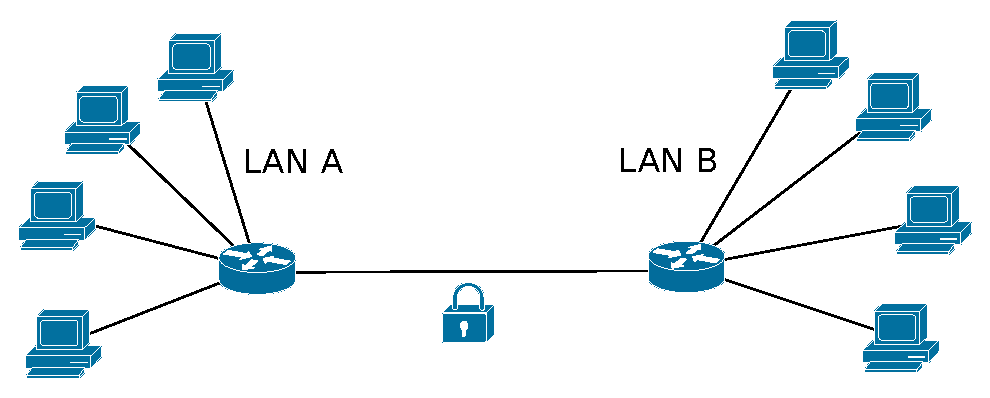
\includegraphics{Diagram_LAN-LAN.eps}
    \caption{Site-to-Site-Szenario}
    \label{fig:site-to-site-szenario}
\end{figure}

\begin{figure}[h!]
    \centering
    \def\svgwidth{\columnwidth}
    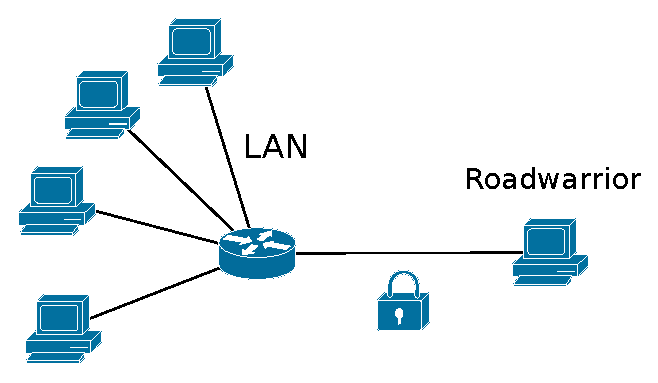
\includegraphics{Diagram_LAN-ROADWARRIOR.eps}
    \caption{Roadwarrior-Szenario}
    \label{fig:roadwarrior-szenario}
\end{figure}


\subsubsection{IPsec unter Linux}
Unter Linux gibt es zwei verschiedene \ac{IPsec}-Stacks.
Es existiert einerseits der KLIPS-Stack, der vom FreeS/WAN-Projekt entwickelt wurde
und auf Route based IPsec basiert.

Des weiteren gibt es den XFRM-Stack, welcher auf Policy based IPsec basiert, jedoch mithilfe eines \ac{VTI}
auch für Route based IPsec genutzt werden kann.

Beide Stacks sind konform zu RFC 2367\footcite[][]{daniel_l._mcdonald_rfc_1998}.

Die Kommunikation mit dem Kernel bezüglich Netzwerkfunktionen geschieht über
den Netlink-Sockel. 
Das ''strongSwan''-Projekt implementiert mit dem Dienst ''charon'' einen \ac{ISAKMP}/IKEv1 und IKEv2-Keying-Daemon
auf Linux.
Die notwendigen Funktionen für die Kommunikation mit dem Kernel sind in ''charon'' im Plugin ''kernel-netlink'' implementiert.
Über Netlink werden auch die \ac{SAD} und \ac{SPD} verwaltet.

\subsubsection{IPsec unter Windows}
Microsoft hat im Laufe der Entwicklungsgeschichte von Windows drei verschiedene
\ac{IPsec}-Implementierungen implementiert, die teilweise parallel existierten.

In der Firewall von Windows existiert eine Implementierung, die Policy-based ist
und daher flexibler ist und es erlaubt Firewall-Regeln zu schreiben, die abhängig davon sind,
ob ein Paket mit \ac{IPsec} geschützt war.

''strongSwan'' implementiert mit ''charon-svc'' einen \ac{ISAKMP}/IKEv1 und IKEv2-Keying-Daemon
auf Windows. Die Kommunikation mit dem Kernel ist dort in den Plugins ''kernel-wfp''
und ''kernel-iph'' implementiert.

\paragraph{Windows Agile VPN Client}
Seit Windows 7 existiert in Windows eine Implementierung von \ac{IPsec} im Netzwerkmnanager,
der den Config-Modus implementiert, sodass Windows als \ac{RW} operieren kann.
Diese Implementierung nutzt eine Route-based-Implementierung, wie in \autoref{subsec:routebased}
erklärt. Diese Implementierung heißt offiziell ''Windows Agile VPN Client'' und
implementiert \ac{PPTP}, \ac{IPsec}+\ac{L2TP}, \ac{SSTP} und \ac{IKE}v2. Sie existiert seit Windows 7.

Die Fähigkeiten dieser Implementierung lässt sich aus den Tabellen im Appendix unter ~\autoref{subsec:featurematrix} ablesen.


\paragraph{IKEEXT}
Windows wird mit einem Dienst namens ''IKEEXT'' ausgeliefert,
welcher genutzt werden kann, um IKE\_SAs und CHILD\_SAs auszuhandeln. Standardmäßig
ist dieser Dienst aktiv und lauscht auf \ac{UDP} Port 500 und 4500.
Diese Implementierung unterstütz den Config-Modus nicht und ist daher nicht für die Benutzung als \ac{RW} geeignet.\footcite[][]{_ipsec_2016}

\paragraph{WFP}
\ac{WFP} ist die grundlegende Technologie im Netzwerkstack von Windows, mit
der \ac{IPsec} im Kernel, sowie die Firewall dort implementiert wurde.
''charon'' kann mit \ac{WFP} mithilfe des ''kernel-wfp''-Plugins kommunizieren
und \acp{SA} und \acp{SP} in die jeweiligen Datenbanken einfügen.

\ac{WFP} hat mehrere Probleme, unter anderem mit virtuellen IP-Adressen,
UDP encapsulation, sowie mit mehreren Traffic Selectors im Transport-Modus.
Des weiteren stellt \ac{WFP} keine Statistiken über die einzelnen \acp{SA} bereit,
was verhindert, dass volumenbasiertes Rekeying und das Auslesen von Nutzungsstatistiken
der \acp{SA} implementiert werden kann.

Aufgrund der Problematik bezüglich virtueller IPs ist es nicht sinnvoll einen \ac{RW}-Client
auf Basis von \ac{WFP} zu erstellen.\footcite[][]{tobias_brunner_kernel-wfp_2014}\footcite[][]{martin_willi_git.strongswan.org_2014}

\paragraph{IPH}
Windows bietet die \ac{IPH}-Funktionen an, die das Verwalten von
\ac{IP}-Adressen, Routen und Geräten erleichtert. ''strongSwan''
nutzt diese Funktionen im ''kernel-iph''-Plugin, um ein Kernel-Interface
für Windows mit diesen Funktionen zu implementieren.


\subsubsection{Route Based}
\label{subsec:routebased}
Route based heißt, dass Pakete, die über das VPN
gesendet werden sollen, in eine virtuelle Netzwerkschnittstelle geroutet werden.
Da gewöhnliches Routing auf Basis der Zieladresse geschieht, unterstützt solche eine solche Implementierung
in der Regel keine \acp{SP}, die nur bestimmte Protokolle oder Ports schützen oder wenn das der Fall ist,
so ist die Kommunikation mit den anderen Ports oder Protokollen nicht mehr möglich,
da jegliche Pakete, die in die Schnittstelle gelangen und von den \acp{SP} nicht zugelassen sind, verworfen werden.

Implementierungen von IPsec auf Endgeräten sind in der Regel Route based, gleichzeitig werden
die ausgehandelten \acp{SP} jedoch weiterhin erzwungen.
Route based \acp{VPN} werden für gewöhnlich dann genutzt, wenn dynamisches Routen genutzt wird,
wie zum Beispiel \ac{BGP}, \ac{ISIS} oder \ac{OSPF}, da beim Verändern der Routen die \acp{SP} nicht verändert
und damit keine neuen CHILD\_SAs ausgehandelt werden müssen. Ein weiterer Vorteil ist, dass Neulinge es leichter haben
den Paketfluss zu verfolgen.

Um zu verhindern, dass der \ac{IKE}-Verkehr über das \ac{VPN} geleitet wird, wird
eine Route für die \ac{IP}-Adresse des Peers in den Routing Table installiert,
die den Verkehr am \ac{VPN} vorbei leitet. Aus diesem Grund ist es auch nicht möglich
mit Route based \ac{IPsec} mit der \ac{IP} des Peers unter der Nutzung von \ac{IPsec} zu kommunizieren.

Eine Möglichkeit Pakete, die nicht von den Policies geschützt werden, nicht ins \ac{VPN} zu leiten und
damit die Kommunikation mit ihnen zu ermöglichen ist \ac{PBR} anzuwenden und ebendiese Pakete
speziell zu markieren und eine andere Routing-Entscheidung zu treffen.

\subsubsection{Policy Based}
\label{subsec:policybased}
Policy based bedeutet, dass die \ac{IPsec}-\acp{SP}, die ausgehandelt wurden, direkt genutzt werden welche Pakete geschützt werden.
Eine solche Implementierung ermöglicht es, \ac{IPsec} zur Absicherung von sehr genau spezifiziertem
Verkehr zu nutzen, wie zum Beispiel nur \ac{ICMP}-Pakete mit Typ 0, Code 0 (Echo Reply), sowie Typ 8 und Code 0 (Echo Request).
Policy based \ac{IPsec} ermöglicht es \ac{IPsec} direkt in den Stack zu integrieren, ohne notwendigerweise die Routen zu verändern.
Um sicherzustellen, dass der \ac{IKE}-Verkehr des \ac{IKE}-Daemons nicht mittels einer \ac{IPsec}-\ac{SA} geschützt wird, was
unter Umständen die Kommunikation zwischen den \ac{IKE}-Daemons verschiedener Systeme verhindern kann, werden bestimmte
Optionen auf dem jeweiligen Netzwerksockel gesetzt, die Pakete, die von diesem Sockel kommen, von den \acp{SP} und \acp{SA}
nicht bearbeitet werden.



\subsubsection{TUN und TAP-Geräte}
TUN- und TAP-Geräte sind virtuelle Netzwerkadapter, die von lokalen Anwendungen
genutzt werden können um vom Kernel \ac{IP}-Pakete oder Ethernet-Rahmen zu empfangen.
Pakete und Rahmen, die der Kernel über ein TUN- oder TAP-Gerät erhält
werden gleich behandelt als wären sie über eine physikalische Schnittstelle empfangen worden.
Sie werden auch gleich verwaltet, so können ihnen zum Beispiel \ac{IP}-Adressen zugewiesen
und Routen über so eine virtuelle Schnittstelle angelegt werden.

\paragraph{TUN-Geräte}
TUN-Geräte sind virtuelle Netzwerkschnittstellen, die auf der Netzwerkschicht arbeiten.
Das heißt, dass sie IP-Pakete senden und empfangen ohne einen darunterliegenden Ethernet-Rahmen.
Das heißt im Umkehrschluss das über ein TUN-Gerät keine Kollisionsdomäne erreichbar ist,
ARP nicht benutzbar ist und das ''next hop''-Feld einer Route in der Routing-Tabelle
keine Bedeutung hat, wenn die Route über ein TUN-Gerät führt.

\paragraph{TAP-Geräte}
TAP-Geräte verhalten sich wie physikalische Ethernet-Schnittstellen.
Das heißt, dass prinzipiell über sie ARP und Ethernet gesprochen werden können
und eine Kollisionsdomäne erreichbar ist. TAP-Geräte können genutzt werden
um eine Brücke zwischen einem lokalen Netzwerk und einem entfernten
Netzwerk über einen \ac{VPN}-Dienst mithilfe eines virtuellen Brückengeräts
zu bauen.
